\documentclass[border=3.14mm,tikz]{standalone}
\usepackage{pgfplots}
\usepackage{xxcolor}
\pgfplotsset{compat=1.15}
\usetikzlibrary{decorations.pathmorphing,decorations.markings}
% Declare nice sphere shading: http://tex.stackexchange.com/a/54239/12440
\pgfdeclareradialshading[tikz@ball]{ball}{\pgfqpoint{0bp}{0bp}}{%
 color(0bp)=(tikz@ball!0!white);
 color(7bp)=(tikz@ball!0!white);
 color(15bp)=(tikz@ball!70!black);
 color(20bp)=(black!70);
 color(30bp)=(black!70)}
\makeatother

% Style to set TikZ camera angle, like PGFPlots `view`
\tikzset{viewport/.style 2 args={
    x={({cos(-#1)*1cm},{sin(-#1)*sin(#2)*1cm})},
    y={({-sin(-#1)*1cm},{cos(-#1)*sin(#2)*1cm})},
    z={(0,{cos(#2)*1cm})}
}}

% Styles to plot only points that are before or behind the sphere.
\pgfplotsset{only foreground/.style={
    restrict expr to domain={rawx*\CameraX + rawy*\CameraY + rawz*\CameraZ}{-0.05:100},
}}
\pgfplotsset{only background/.style={
    restrict expr to domain={rawx*\CameraX + rawy*\CameraY + rawz*\CameraZ}{-100:0.05}
}}

% Automatically plot transparent lines in background and solid lines in foreground
\def\addFGBGplot[#1]#2;{
    \addplot3[#1,only background, opacity=0.25] #2;
    \addplot3[#1,only foreground] #2;
}

% attempt to do similar things for discrete plots
\def\addFGBGSampleplot[#1]#2;{
    %\addplot3[#1,only background,gray!50] #2;
    \addplot3[#1,only foreground] #2;
}


\newcommand{\ViewAzimuth}{-30}
\newcommand{\ViewElevation}{30}

\tikzset{spring/.style={decorate,decoration={aspect=0.5,amplitude=1.5mm, segment
length=1.5mm}}}
% pgfmanual p. 1087
\pgfdeclareradialshading{ballshading}{\pgfpoint{-10bp}{10bp}}
 {color(0bp)=(cyan!15!white); color(9bp)=(cyan!75!white);
 color(18bp)=(cyan!70!black); color(25bp)=(cyan!50!black); color(50bp)=(black)}

\pgfdeclareplotmark{crystal ball}{\pgfpathcircle{\pgfpoint{0ex}{0ex}}{2ex}
  \pgfshadepath{ballshading}{0}
  \pgfusepath{}}
\begin{document}
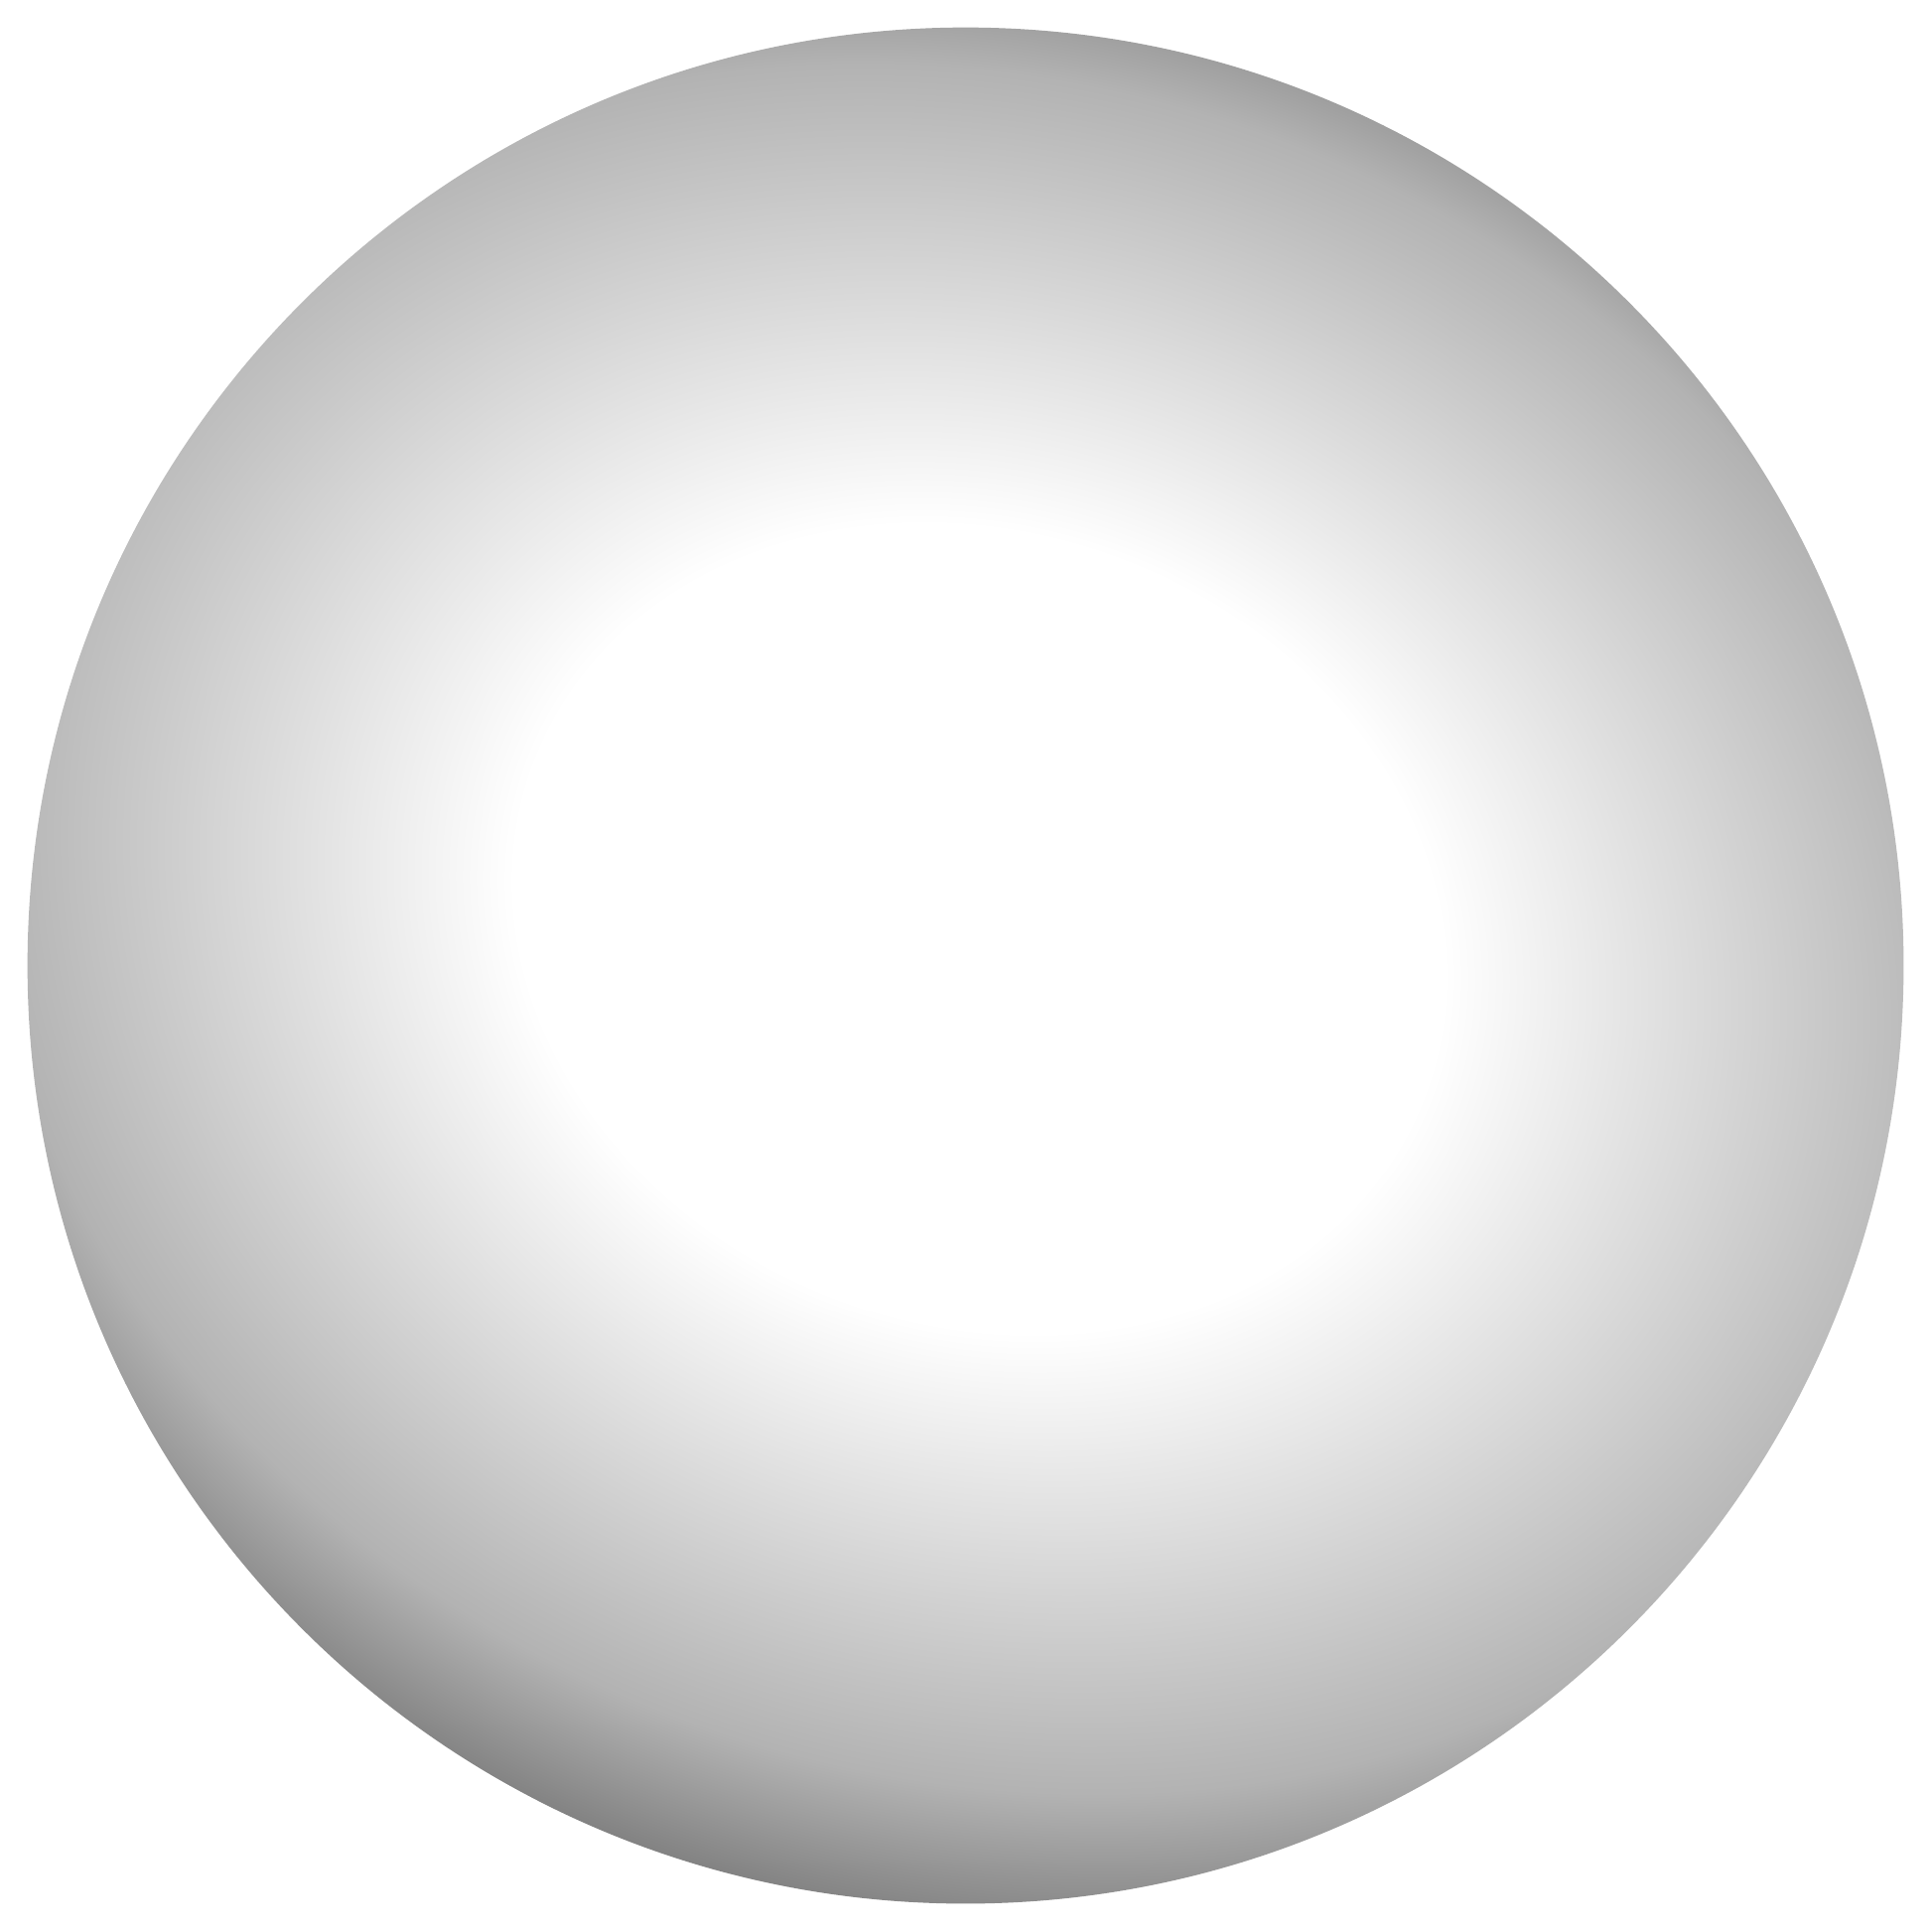
\begin{tikzpicture}
    % Compute camera unit vector for calculating depth
    \pgfmathsetmacro{\CameraX}{sin(\ViewAzimuth)*cos(\ViewElevation)}
    \pgfmathsetmacro{\CameraY}{-cos(\ViewAzimuth)*cos(\ViewElevation)}
    \pgfmathsetmacro{\CameraZ}{sin(\ViewElevation)}
    \pgfmathsetmacro{\R}{12}
    \path[use as bounding box] (-\R,-\R) rectangle (\R,\R); % Avoid jittering animation
    % Draw a nice looking sphere
    \begin{scope}
        \clip (0,0) circle (\R);
        \begin{scope}[transform canvas={rotate=-20}]
            \shade [ball color=white] (0,0.5) ellipse (\R*1.8 and \R*1.5);
        \end{scope}
    \end{scope}
    \begin{axis}[
        hide axis,
        view={\ViewAzimuth}{\ViewElevation},     % Set view angle
        every axis plot/.style={very thin},
        disabledatascaling,                      % Align PGFPlots coordinates with TikZ
        anchor=origin,                           % Align PGFPlots coordinates with TikZ
        viewport={\ViewAzimuth}{\ViewElevation}, % Align PGFPlots coordinates with TikZ
    ]
        % plot latitude circles
        \pgfplotsinvokeforeach{-75,-65,...,75}
        {\addFGBGplot[spring,domain=0:2*pi, samples=51, samples y=1]
        ({\R*cos(#1)*cos(deg(x))}, {\R*cos(#1)*sin(deg(x))}, {\R*sin(#1)});}
        % plot longitude circles
        \pgfplotsinvokeforeach{0,15,...,150}
        {\addFGBGplot[spring,domain=0:2*pi, samples=51, samples y=1]
        ({\R*cos(#1)*cos(deg(x))}, {\R*sin(#1)*cos(deg(x))}, {\R*sin(deg(x))});     
        }
        % plot longitude circles
        \pgfplotsinvokeforeach{0,15,...,330}
        {\addFGBGSampleplot[only marks,mark=crystal ball,samples at={-75,-65,...,75}]
        ({\R*cos(#1)*cos(x)}, {\R*sin(#1)*cos(x)}, {\R*sin(x)});        
        }
    \end{axis}
\end{tikzpicture}
\end{document}